% !TeX spellcheck = de_DE
%-----------------------------------------------------
%  Introduction
%-----------------------------------------------------


\section{서론}
\subsection{연구의 필요성}

천체망원경이 대중화됨에 따라 일반인들도 소형 천체망원경과 DSLR (Digital Single Lens Replex) 카메라나 CCD 등을 이용하여 사진 관측을 하는 경우가 있다. 대부분의 천체관측은 해가 진 야간에 날씨가 맑을 경우에만 가능하다보니 시간적으로 매우 제한적이다. 또한 지상에서의 천체관측은 대기 영향에 의해 많은 어려움이 따른다. 대기의 영향을 최소화 하기 위해서는 관측 대상의 고도가 높은 시각에 관측을 하는 것이 유리하다. 

또한 사진 관측에서 중요한 요소 중 하나는 초점을 정확하게 조절하는 것이다. 사진 관측시 온도 변화로 인해 경통의 팽창, 수축으로 인하여 정확하게 조절해 놓은 초점이 변하는 경우도 있다. 최근에는 이러한 문제를 해결하기 위해 컴퓨터를 이용하여 정확한 제어를 통해 짧은 시간안에 효율적인 관측을 진행하고자 노력하고 있다. Persha (2001)는 주위 온도에 따라서 초점이 변화한다는 점을 보완하고자 이를 보정할 수 있도록 온도 보상 초점 조절 방법을 연구하였다.\cite{persha2001temperature} 


%천체 관측은 천체 망원경이 대중화됨에 따라 여러 사람들이 시도하는 경우가 많아졌다. 하지만 천체관측을 할 시에는 여러 가지 변수가 존재하여, 천체관측을 어렵게 하는 경우가 있다. 천체 관측을 하는 데 중요한 요소 중 하나는 초점을 정확하게 맞추는 것이다. 초점이 얼마나 정확하게 맞았는 지에 따라서 천체관측한 사진의 상이 얼마나 정확하게 나왔는지가 달라질 뿐만이 아니라 장시간 노출을 하여 사진을 촬영해야 하는 밤에 경우 초점이 맞지 않으면 그 차이가 더욱 두드러지게 나타나게 된다. 최근에는 이러한 문제를 해결하기 위해 컴퓨터를 이용하여 정확한 제어를 통해 짧은 시간안에 효율적인 관측을 진행하고자 노력하고 있다.

\begin{figure}[h]
	\begin{center}
		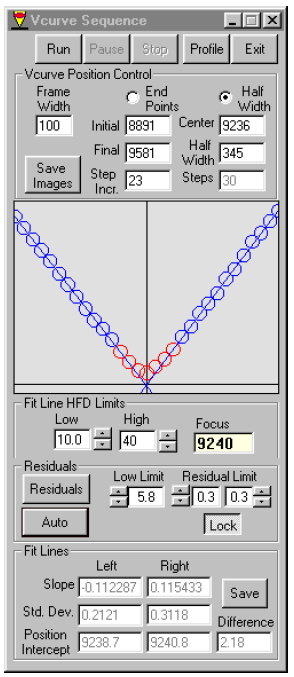
\includegraphics[width = 5cm]{V-curve}
	\end{center}
	\caption{FocusMAX 소프트웨어를 이용하여 FWHM 값의 V-curve를 얻어 초점을 결정하는 모습. \cite{weber2001fast}}
	\label{V-curve}
\end{figure}

사진 관측시 천체망원경의 초점 조절을 정밀하게 하기 위하여 다음과 같은 방법을 사용하고 있다. 

첫째는 사진에서의 대기의 상태에 의한 별의 점퍼짐 함수의 FWHM (Full Width Half Maximum) 값을 활용하여 V-curve를 그리는 방법이다. \textrm{Figure}. \ref{V-curve}은 FocusMax 소프트웨어로 포커서를 움직이며 별의 점퍼짐 함수의 FWHM을 구하여 V-curve를 얻어 최적의 초점을 찾는 모습을 나타낸다. 이 방법을 활용할 경우 어떤 상황에서도 꽤 정확한 결과를 얻을 수 있지만, 이는 별의 플럭스가 정규분포로 퍼져있어야 정확한 결과를 얻을 수 있다. 만약 별이 포화되어 점퍼짐 함수가 정규분포와 모양이 다른 경우에는 HFD (Half Flux Diameter) 값을 이용할 수 있지만 시잉(seeing)의 영향으로 에러가 발생하여 초점을 조절하는데 어려움을 겪는다. 

\begin{figure}[h]
	\begin{center}
		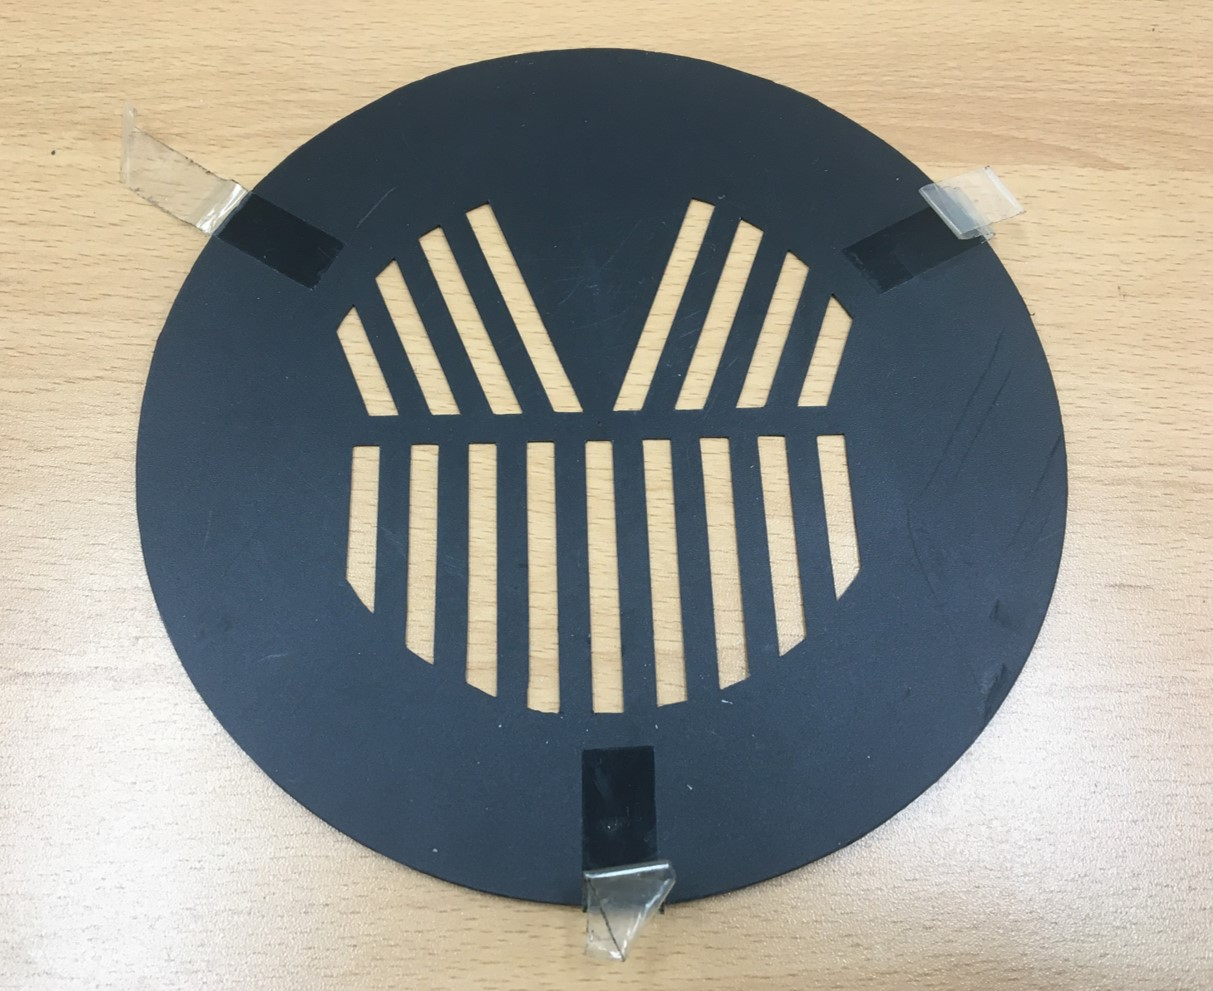
\includegraphics[width = 8cm]{bahtinov1}
	\end{center}
	\caption{PP(Polypropylene) 소재의 파일 표지를 잘라서 만든 바흐티노프 마스크}
	\label{bahtinov}
\end{figure}

이런 어려움을 개선하기 위해서 다른 방법으로 마스크를 활용하는 방법이 주목받고 있다. 천체관측에서 초점 조절에 사용하는 하트만 마스크(Hartmann mask)와 바흐티노프 마스크(Bahtinov mask)가 있다. 바흐티노프 마스크는 러시아의 아마추어 천문학자인 바흐티노프가 고안한 마스크 중 하나로, 기존에 사용하던 하트만 마스크의 여러 단점을 보완하였기 때문에 이후 주류가 된 마스크의 종류이다. 두 마스크 모두 빛의 회절 현상을 이용한다는 공통점이 있지만, 천체관측에서는 바흐티노프 마스크가 더 포괄적으로 사용된다. 마스크를 이용하면 점퍼짐 함수의 FWHM 값을 구하여 초점을 조절하는 것에 비해 대기에 의한 영향을 덜 받는다는 것이 장점이며, 제작 및 관리에도 용이하기 때문에 천체망원경의 원격 제어에 알맞은 특징들을 지니고 있다. 

빛의 회절은 직진하던 빛이 좁은 틈, 슬릿이나 장애물을 통과할 때 물체의 뒤편까지 빛이 나가는 현상으로, 슬릿의 폭이 좁을수록 회절이 잘 일어난다. 바흐티노프 마스크는 Figure. \ref{bahtinov}와 같이 방향이 어긋나있는 세 줄의 회절 슬릿들이 일렬로 나있는 모양을 가지고 있으며, 평행 광선인 별에서 오는 빛이 이러한 모양의 슬릿을 통과하면 빛은 좁은 틈에서 회절하게 된다. 빛은 좁은 방향으로 많이 회절하기 때문에 슬릿을 통과한 빛은 통과한 슬릿에 수평한 방향의 선 모양 상을 만들게 된다. 초점이 올바르지 않은 경우에는 평행광이 한점에 모이지 않기 때문에 세 개의 선이 한 점에서 만나지 않지만, 초점이 정확하게 맞추어진 경우에는 상들이 한 점에서 모이기 때문에 세 개의 선이 한 점에서 만나게 된다.

바흐티노프 마스크는 빛의 회절을 이용하여 초점이 정확한지 여부를  쉽고 빠르게 알 수 있기 때문에 관측시간이 중요한 천체망원경의 초점을 맞추는 데 안성맞춤이다. 회절 슬릿을 이용하기 때문에 아주 밝은 별로만 초점 검출을 할 수 있다는 단점을 가지고 있지만 상대적으로 노출의 시간을 늘리는 밤에 천체관측을 할 때는 바흐티노프마스크가 좋은 선택이라고 할 수 있다.

본교 보조관측실은 자동으로 개폐되는 슬라이딩 루프(sliding roof)가 있어, 이곳에 소형 천체망원경을 고정하여 설치해 놓고 관측을 진행하고 있다. 천체망원경의 완전 자동화가 가능하다면 제한된 관측 가능 시간에 관측 성공률이 높아질 것이다. 실제로 여러 천문대에서 천체망원경 자동화를 위해 노력하고 있고, Zhang 등(2016)은 남극에 위치한 망원경의 자동관측에 대해 연구하였다 .\cite{Zhang2016}

Budding (1995) 또한 뉴질랜드 카터 천체관측소(Carter)에 자동화된 소형 천체망원경을 설치하여 운영하면서 소형 천체망원경을 원격제어할 수 있도록 네트워크를 활용하면 일반적인 천체관측에 비해 비용측에서 큰 이득을 보며, 편의성또한 증대할 수 있다고 주장하였다.\cite{budding1995global} 



\subsection{연구 목적}

%본 연구에서는 은형 천체망원경의 자동화를 위한 효율적인 초점조절방식인 바흐티노프마스크의 제어를 효율적으로 할 수 있도록 하며, 이를 위하여 소형 천체망원경에서 사용할 수 있는 덮개를 제작하여 실제 관측에 적용하는 것을 목적으로 한다. 

본 연구에서는 경기과학고등학교 보조관측실에 설치되어 있는 소형 천체망원경의 자동화를 위한 장치와 이를 구동할 수 있는 소프트웨어를 개발하는 것이 그 목적이다. 소형 천체망원경의 원격 제어 및 자동화를 위해서는 돔 컨트롤, 전원 컨트롤, 마운트 컨트롤, 초점 컨트롤, 망원경 덮개 컨트롤, 이슬 제거를 위한 열선 컨트롤 등이 스스로 동작하거나 컴퓨터로 제어가 가능해야 한다. 현재 본교 보조관측실에 설치된 소형 천체망원경의 자동화를 구현하기 위해서 필요한 것들을 \textrm{Table}. \ref{controll}에 나타내었다.

\begin{table}[htbp]
	\caption{보조관측실에 설치된 소형 천체망원경의 자동화를 위해 필요한 컨트롤}
	\label{controll}
	\resizebox{\textwidth}{!}{%
		\begin{tabular}{c|c|c|c}
			\hline	\toprule
			컨트롤 & 구축 여부 & 제어 방법 & 비고
			\\ 		\hline	\toprule
			슬라이딩 루프 컨트롤   &  구축됨     & 아두이노, 릴레이스위치, 전용 소프트웨어로 제어   & 
			\\		\hline
			마운트 컨트롤    &  구축됨    &  제조사 제공 망원경 컨트롤 시스템, ASCOM 제어    &
			\\		\hline
			전원 컨트롤   &  별도로 구축됨     & 아두이노, 릴레이스위치, 전용 소프트웨어로 제어   & GS-system에 포함
			\\		\hline
			모터 포커서 컨트롤    &  별도로 구축됨    & GS-touch, ASCOM 제어 & GS-system에 포함          
			\\ 		\hline
			망원경 덮개 컨트롤    &  구축안됨    &  & GS-system에 포함
			\\ 		\hline
			이슬 제거용 열선 컨트롤    &  별도로 구축됨    & 수동 전기 회로, 수동 제어 & GS-system에 포함
			\\ 		\hline	\toprule
		\end{tabular}%
	}
\end{table}

개발된 시스템의 이름은 경기과학고등학교의 영문명인 Gyeonggi Science high school for the gifted 중에서 GS를 따와서 GS-system이라 명명하였다. GS-system은 기기의 전원 컨트롤, 마운트 컨트롤, 망원경 덮개 컨트롤, 초점 조절, 이슬 제거를 위한 열선 컨트롤 등을 포함하고 있으며, 이것들을 컴퓨터로 컨트롤 하는데 성공한다면 인터넷을 통해 컴퓨터를 원격 조정하는 방법이나 컴퓨터 프로그램으로 미리 지정한 스케줄에 따라 관측기기들을 구동을 예약하는 방법으로 소형 천체망원경의 자동화를 구현할 수 있게 된다. 

GS-system은 바이폴라 스테핑 모터를 사용하는 모터 포커서를 제어하기 위해 제작하였던 GS-touch (Gyeonggi Science high school for the gifted touch) 를 응용하여 ASCOM (Astronomy Common Object Model) 지원 소프트웨어와 호환되도록 개발하였다. 

본 연구에서 제시하는 연구 문제는 다음과 같다:

\begin{enumerate}
	
	\item 천체망원경 자동화를 위한 전원 스위치, 모터 포커서, 망원경 덮개, 이슬 제거용 열선 등을 제작할 수 있는가?
	\item 천체망원경 자동화를 위한 전원 스위치, 모터 포커서, 망원경 덮개, 이슬 제거용 열선 등을 제어할수 있는 회로를 구성할 수 있는가?
	\item 천체망원경 자동화를 위한 전원 스위치, 모터 포커을, 망원경 덮개, 이슬 제거용 열선 등을 제어할수 있는 ASCOM 호환 소프트웨어를 개발할 수 있는가?
	
\end{enumerate}

Godoy 등(2018)또한 본 연구의 연구 목적과 연구 문제를 제시하였으며, 이를 실제로 연구에 활용하였으며, 천체망원경의 원격제어에 성공하였다. \cite{godoy2018control} 또한, 본 결과들을 통해 앞으로 천체망원경의 자동화 시스템을 제작하려는 사람들에게 도움이 되고자 한다.